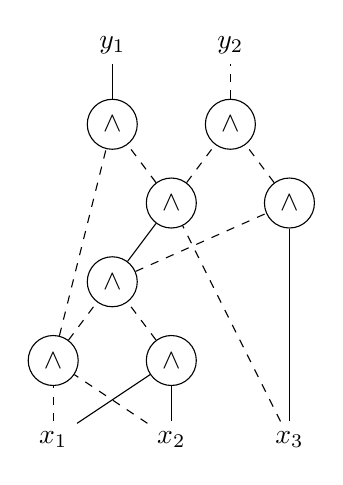
\begin{tikzpicture}[]
    % First rank with three nodes called x_1, x_2, x_3
    \node[draw=none] (x_1) at (0,0) {$x_1$};
    \node[draw=none] (x_2) at (1.5,0) {$x_2$};
    \node[draw=none] (x_3) at (3,0) {$x_3$};
    
    % Second rank with two nodes above x_1 and x_2 called x_4, x_5
    \node[draw, circle] (x_4) at (0.00, 1) {$\land$};
    \node[draw, circle] (x_5) at (1.50, 1) {$\land$};
    
    % Third rank with one node called x_6
    \node[draw, circle] (x_6) at (0.75, 2) {$\land$};

    % Fourth rank with two nodes called x_7 and x_8
    \node[draw, circle] (x_7) at (1.5, 3) {$\land$};
    \node[draw, circle] (x_8) at (3, 3) {$\land$};

    % Fifth rank with two nodes called x_9 and x_10
    \node[draw, circle] (x_9) at  (0.75,4) {$\land$};
    \node[draw, circle] (x_10) at (2.25,4) {$\land$};

    % Sixth rank with two nodes called y_1 and y_2
    \node[draw=none] (y_1) at (0.75,5) {$y_1$};
    \node[draw=none] (y_2) at (2.25,5) {$y_2$};
    
    % Connections
    \draw[dashed] (x_1) -- (x_4);
    \draw (x_1) -- (x_5);
    
    \draw[dashed] (x_2) -- (x_4);
    \draw (x_2) -- (x_5);

    \draw[dashed] (x_3) -- (x_7);
    \draw (x_3) -- (x_8);

    \draw[dashed] (x_4) -- (x_9);
    \draw[dashed] (x_4) -- (x_6);

    \draw[dashed] (x_5) -- (x_6);

    \draw (x_6) -- (x_7);
    \draw[dashed] (x_6) -- (x_8);

    \draw[dashed] (x_7) -- (x_9);
    \draw[dashed] (x_7) -- (x_10);

    \draw[dashed] (x_8) -- (x_10);

    \draw (x_9) -- (y_1);

    \draw[dashed] (x_10) -- (y_2);
    
\end{tikzpicture}
